%% This is file `elsarticle-template-1-num.tex',
%%
%% Copyright 2009 Elsevier Ltd
%%
%% This file is part of the 'Elsarticle Bundle'.
%% ---------------------------------------------
%%
%% It may be distributed under the conditions of the LaTeX Project Public
%% License, either version 1.2 of this license or (at your option) any
%% later version.  The latest version of this license is in
%%    http://www.latex-project.org/lppl.txt
%% and version 1.2 or later is part of all distributions of LaTeX
%% version 1999/12/01 or later.
%%
%% Template article for Elsevier's document class `elsarticle'
%% with numbered style bibliographic references
%%
%% $Id: elsarticle-template-1-num.tex 149 2009-10-08 05:01:15Z rishi $
%% $URL: http://lenova.river-valley.com/svn/elsbst/trunk/elsarticle-template-1-num.tex $
%%
%%\documentclass[preprint,12pt]{elsarticle}
\documentclass[preprint,12pt,3p]{elsarticle}

%% Use the option review to obtain double line spacing
%% \documentclass[preprint,review,12pt]{elsarticle}

%% Use the options 1p,twocolumn; 3p; 3p,twocolumn; 5p; or 5p,twocolumn
%% for a journal layout:
%% \documentclass[final,1p,times]{elsarticle}
%% \documentclass[final,1p,times,twocolumn]{elsarticle}
%% \documentclass[final,3p,times]{elsarticle}
%% \documentclass[final,3p,times,twocolumn]{elsarticle}
%% \documentclass[final,5p,times]{elsarticle}
%% \documentclass[final,5p,times,twocolumn]{elsarticle}

%% The graphicx package provides the includegraphics command.
\usepackage{graphicx}
%% The amssymb package provides various useful mathematical symbols
\usepackage{amssymb}
%% The amsthm package provides extended theorem environments
%% \usepackage{amsthm}

%% The lineno packages adds line numbers. Start line numbering with
%% \begin{linenumbers}, end it with \end{linenumbers}. Or switch it on
%% for the whole article with \linenumbers after \end{frontmatter}.
\usepackage{lineno}

\usepackage{gensymb}
\usepackage{siunitx}
\usepackage{amsmath}
\usepackage{todonotes}
\usepackage{blkarray}

%% natbib.sty is loaded by default. However, natbib options can be
%% provided with \biboptions{...} command. Following options are
%% valid:

%%   round  -  round parentheses are used (default)
%%   square -  square brackets are used   [option]
%%   curly  -  curly braces are used      {option}
%%   angle  -  angle brackets are used    <option>
%%   semicolon  -  multiple citations separated by semi-colon
%%   colon  - same as semicolon, an earlier confusion
%%   comma  -  separated by comma
%%   numbers-  selects numerical citations
%%   super  -  numerical citations as superscripts
%%   sort   -  sorts multiple citations according to order in ref. list
%%   sort&compress   -  like sort, but also compresses numerical citations
%%   compress - compresses without sorting
%%
%% \biboptions{comma,round}

% \biboptions{}

\journal{ISPRS J. Photogram. Remote Sens.}

\begin{document}

\begin{frontmatter}

%% Title, authors and addresses

\title{Pushing the limits of geomorphic change detection by error propagation in 3D topographic point clouds}

%% use the tnoteref command within \title for footnotes;
%% use the tnotetext command for the associated footnote;
%% use the fnref command within \author or \address for footnotes;
%% use the fntext command for the associated footnote;
%% use the corref command within \author for corresponding author footnotes;
%% use the cortext command for the associated footnote;
%% use the ead command for the email address,
%% and the form \ead[url] for the home page:
%%
%% \title{Title\tnoteref{label1}}
%% \tnotetext[label1]{}
%% \author{Name\corref{cor1}\fnref{label2}}
%% \ead{email address}
%% \ead[url]{home page}
%% \fntext[label2]{}
%% \cortext[cor1]{}
%% \address{Address\fnref{label3}}
%% \fntext[label3]{}


%% use optional labels to link authors explicitly to addresses:
%% \author[label1,label2]{<author name>}
%% \address[label1]{<address>}
%% \address[label2]{<address>}

\author[1]{Lukas Winiwarter}
\author[1,2]{Katharina Anders}
\author[1,2]{Bernhard Höfle}
\address[1]{3DGeo Research Group, Institute of Geography, Heidelberg University, Germany}
\address[2]{Institute for Scientific Computing (IWR), Heidelberg University, Germany}

\begin{abstract}
%% Text of abstract
Detection and quantification of geomorphic surface change is an important part of natural hazard management. For change detection in 3D topographic point clouds, acquired using e.g. terrestrial laser scanning (TLS), random and systematic noise has to be separated from the change signal. In point cloud differencing, the multiscale model-to-model cloud comparison (M3C2) approach is commonly applied, which provides a statistical significance test based on the local variance of the point cloud neighbourhood. This test is valid on planar surfaces sampled with a constant uncertainty level, and includes a single term corresponding to alignment uncertainty. 

We extend this test by propagating the measurement and alignment uncertainties to achieve 3D covariance information on a per-point level, combining sensor knowledge and residuals from the alignment. Then, we quantify the Level of Detection, the minimum detectable change, using a 3D statistical significance test. 
We verify our method in two simulated scenarios and apply it on a TLS time series of a rock glacier at two different timespans of 3 weeks and 1 year respectively. 
In the three weeks period, we manage to detect significant change at an additional 53\% of
spatial locations, corresponding to a volume of \SI{217}{m$^3$}, when compared to the baseline. 
\end{abstract}

\begin{keyword}
Level of Detection \sep t-Test \sep Signal-Noise-Separation \sep Terrestrial Laser Scanning \sep Rock glacier
%% keywords here, in the form: keyword \sep keyword

%% MSC codes here, in the form: \MSC code \sep code
%% or \MSC[2008] code \sep code (2000 is the default)

\end{keyword}

\end{frontmatter}

%%
%% Start line numbering here if you want
%%
\linenumbers


%%\defcitealias{gum}{JCGM, 2008}

%% main text
\section{Introduction}
\label{sec:introduction}

The Earth's surface is subject to constant change. Some of these changes have a local-level impact on geomorphology. To study the phenomena causing these changes, and to monitor and predict mass movements, remote sensing methods are employed \citep{Brodu_Lague_2012, Eitel2016}. Laser~scanning is such a method, sampling three-dimensional points representing the surface. Depending on the measurement platform, the measurement is referred to as airborne laser scanning (ALS), laser scanning from unmanned areal vehicles (ULS) or terrestrial laser scanning (TLS).


The result of laser scanning a surface is a three-dimensional point cloud, an unordered, irregular set of 3D coordinates. Additional attributes such as the signal strength or information of the returned laser pulse shape may be recorded for every point \citep{Otepka_2013}. The measurement process, often based on the flight time of the emitted laser pulse, is subject to uncertainties\footnote{We take care to use the term "uncertainty" as defined in the \emph{Guide to the expression of uncertainty in measurement}: "The uncertainty [...] reflects the lack of exact knowledge of the value of the measurand" \citep{gum}, in contrast to "error", which is "an idealized concept and [...] cannot be known exactly" \citep{gum}. }. These stem from the sensor itself (e.g. synchronization between sender and reciever, reciever noise, ...), the medium of transmission (air; temperature, pressure, humidity) and the sampled object (local incidence angle, reflectance, sub-footprint roughness). Since the area illuminated by the laser is not infinitesimal, some angular ambiguity is also introduced \citep{Lichti_Jamtsho_2006, pfeifer2007investigating, Zame_2014, Wujanz_2017}.

\subsection{Point cloud distance metrics}

There is no straightforward comparison of point clouds from two different points in time (epochs), since the second acquisition will never have the exact same point distribution on the surface as the first one. Therefore, no one-to-one point homology can be established, and point-to-point distances cannot be directly calculated. Different methods to solve this problem have been established, which are presented shortly in this section. Furthermore, multitemporal datasets have to be aligned before change analyses can be carried out, which is commonly done using either signalled markers or defined stable areas, where the discrepancies between the two datasets are minimized. This process introduces further uncertainties, which are correlated for the points of a dataset. This correlation can also be considered. All of the presented point cloud distance metrics deal with two datasets. For change analyses, this is the atomic unit of a bitemporal analysis. Multi-temporal analyses such as \citet{anders20204d} use this atomic unit to extract 4D information.

The most prominent method involves the creation of a regular representation of the terrain, i.e. a digital terrain model (DTM) of each epoch. Subsequently, the difference between the DTMs is calculated, giving a DTM of Difference (DoD), which represents the vertical offset at every pixel location. The downsides of this method are the constant direction of analysis (parallel to the z-Axis), the aggregation of points into a regular raster (which results in a loss of information), and the inability to represent change that is happening in the x/y-plane.

Based on the full point cloud, a first approach is the Cloud-To-Cloud (C2C) distance. It reports the minimal euclidean distance between a point from Epoch 1 and the closest point from Epoch 2. This approach especially suffers from single outliers, as they may have an impact on multiple distances, if the outlier is much closer to the point cloud of the compared epoch. Furthermore, distances are generally underestimated, as the direction of analysis is always chosen to be towards the closest neighbour.

The Cloud-To-Mesh (C2M) distance requires a model (i.e., a triangular irregular network, or triangular mesh) to be created from one of the datasets. Then, the distance can be calculated orthogonal to the respective triangle face. If the mesh is oriented, this also allows the calculation of signed distances, so the separation of volume gain from volume loss. Depending on the resolution of the dataset that is used for the model, changes in different scales may become visible. In comparison to the C2C distance, the triangle normal vector gives a more robust direction of analysis.

Similarly, both datasets can be replaced by a model. The Mesh-to-Mesh (M2M) distance allows the calculation of volumes between the two meshes, which can be of particular interest in geomorphology. This volume is also symmetric, i.e. the order of the input point clouds does not influence the result, which is not the case for the previously mentioned cloud-based metrics. As with the C2M distance, a sign can be assigned if the mesh intersection forms multiple volumes.

Finally, the multiscale model-to-model cloud comparison \citep[M3C2,][]{Lague2013} is the current state-of-the art in geomorphic point cloud change analysis \citep{Zahs2019}. For a subset (often called the \emph{core points}) of the reference point cloud, the local normal vector is estimated based on a neighbourhood of maximum planarity. Then, a query cylinder is created, using the normal vector as its axis. The points from both epochs are aggregated within the cylinder and their respective centers of gravity (CoGs) are calculated. The distance between the CoGs is then projected onto the cylinder axis, and used as distance measure between the point clouds at the location of the core point (Figure~\ref{fig:m3c2}) \citep{Lague2013}.

\begin{figure}
    \centering
    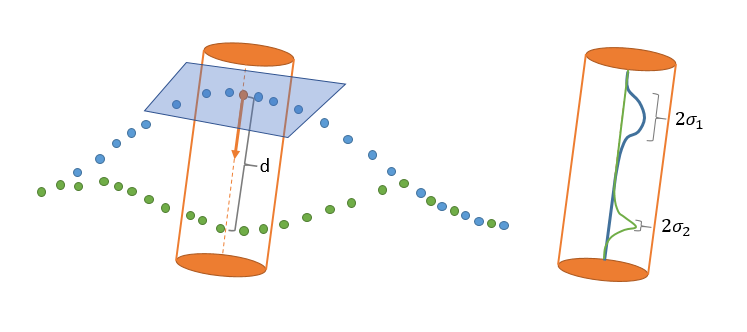
\includegraphics[width=0.9\linewidth]{figs/m3c2.png}
    \caption{M3C2 point cloud distance. Two epochs (blue and green) are compared by estimating a local plane (blue) at a core point (orange) in the reference epoch, and then aggregating the points of the two epochs in a search cylinder aligned with the normal vector of the plane. The distance between the centers of gravity, projected onto the cylinder axis, is the distance $d$ (left). Additionally, the standard deviations of the point distributions along the axis are calculated as $\sigma_1$ and $\sigma_2$ (right).}
    \label{fig:m3c2}
\end{figure}

Additionally, the sample variance of the local neighbourhood within the query cylinder is estimated for each epoch (Figure~\ref{fig:m3c2}, right). This measure, which is also projected onto the cylinder axis, is used as proxy for the accuracy of the CoG, and used in a t-Test. The null hypothesis is that the projection of the two CoGs, which represent mean values, is zero. Equation~\ref{eqn:t-test} gives the test statistic that is compared to the respective quantile of the F-distribution. It can also be reformulated to give information about the smallest change that can be distinguished from noise, commonly referred to as the Level of Detection (LoDetection), as shown in Equation~\ref{eqn:lod}. The value of 1.96 stems from the 95\% quantile of the F-distrubtion with degrees of freedom $n_1, n_2 > 30$, and is commonly used \citep{borradaile2003statistics}.

\begin{equation}
    t^2 = \sqrt{\frac{\sigma_1^2}{n_1} + \frac{\sigma_2^2}{n_2}} + reg.
    \label{eqn:t-test}
\end{equation}

\begin{equation}
    LoDetection_{95\%} = 1.96 \left( \sqrt{\frac{\sigma_1^2}{n_1} + \frac{\sigma_2^2}{n_2}} + reg. \right)
    \label{eqn:lod}
\end{equation}


\subsection{Geomorphic surface changes}
(tbd...) \todo{Braucht es das überhaupt?}

\section{Methods and Experiments}
\label{sec:methods}

In this contribution, we present a novel change detection and quantification method for 3D point clouds. We extend the state-of-the-art M3C2 method by incorporating knowledge about the uncertainty of individual points, stemming from the measurement and alignment. This allows weighing the individual observations in the CoG calculation, and the use of propagated variance for statistical testing. Since we propagate errors\footnote{here: uncertainties, but 'error propagation' is more commonly used than 'uncertainty propagation'}, we refer to the results our method as either the "CoG-EP" for the CoG or "LoDetection-EP" for the minimum quantifiable change.

We present our method by three different additions to the standard M3C2 LoDetection quantification. First, we investigate how observations with different standard deviations influence the LoDetection by simulating a random sampling of a flat surface. Next, we show how non-planar geometries generally increase the baseline LoDetection, and how we can circumvent this phenomenon. We also introduce the usage of a full 3D statistical test for the analysis and show its validity by laser scan simulation. Finally, we show how we can estimate the uncertainty stemming from the alignment of two point clouds from two different epochs by using information from the alignment process (an ICP-variant, see Section~\ref{sec:methods-c}), and how we can integrate this into the quantification of the LoDetection. We then apply our method to a real-world TLS dataset of a rock glacier on two different time spans (1 year and 3 weeks), highlighting the differences and similarities to the baseline.


\subsection{(a) Merging of scan positions}
\label{sec:methods-a}
In the first experiment, we evaluate how measurements with different accuracies can be combined into a mean with the lowest variance, i.e. a BLUE (Best Linear Unbiased Estimator) of the mean. For this, we sample $n$ points in 1D (e.g. distance measurements) from a normal distribution $N_1 (0, \sigma_1^2)$ and combine them with $m$ points sampled from another normal distribution $N_2(0, \sigma_2^2)$. We then calculate the baseline by taking the mean value of the merged $m+n$ points, which has expectation 0. Its sample variance (estimated from the sampled data) is further used to estimate the baseline LoDetection. 

If we have knowledge on the distributions the individual points were sampled from, we can instead calculate a weighted mean (with weights $1/\sigma_1^2$ for the first $n$ and $1/\sigma_2^2$ for the other $m$ points), which also has expectation 0. However, the variance can be predicted by calculating the average variance as $1/(m+n) (n\sigma_1^2 + m\sigma_2^2)$, again allowing the derivation of a LoDetection.
Both Levels of Detection are based on statistical tests, namely a t-Test of equal means, the baseline using the sample variance as calculated from the data and the novel method using the a-priori variance from knowledge on the underlying distribution. The exact choice of siginificance level is secondary, as long as the information on the level is preserved \citep{taylor1997introduction, lane2003estimation}. We therefore estimate the LoDetection at 95\% confidence, as done by \citet{Lague_2013}.

To test the correctness of the LoDetection-EP, we sample and calculate the distance of these means to the means of an independent sampling of the same composition (representing a second epoch, where no change has occurred) 1000 times. In this Monte-Carlo approach, we can then quantify the central 95\% of the calculated distances by taking the 0.025- and the 0.975-quantiles of the distances, corresponding to 5\% outliers.

This experiment is carried out for different values of n while keeping m constant. This simulates an increasing number of scan positions that are further away (i.e., less accurate) or in general, an increasing number of observations with a higher uncertainty.

\subsection{(b) Non-planar objects}
\label{sec:methods-b}
A second experiment shows the resilience of our method to non-planar objects. As shown in Figure~\ref{fig:setup_b}, we assume a scan of the intersection of two planes, where the laser beam is orthogonal to the intersection line. The intersection angle is then varied from the two planes forming a flat surface (0\degree) to them being almost normal to the view direction (90\degree). 
The normal vector for change analysis is kept constant towards the scanner. Therefore, with increasing intersection angle, the sample variance along this change axis increases, which leads to an overestimation of the LoDetection in the baseline method. By using the averaged measurement accuracy (which is in this case identical to the accuracy of a single measurement, as only one scan position is assumed), the LoDetection-EP can be alternatively derived for our method.

\begin{figure}
    \centering
    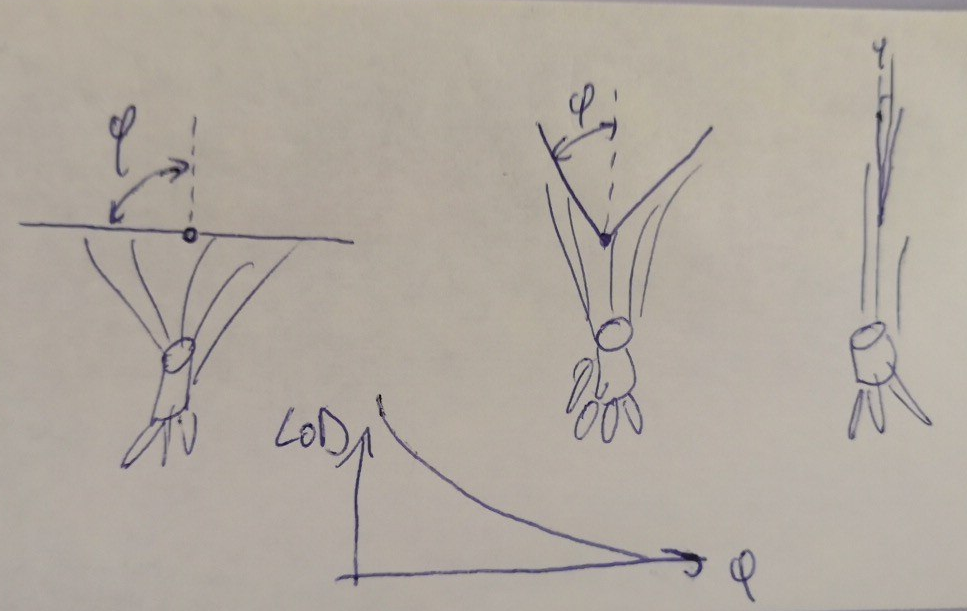
\includegraphics[width=0.9\linewidth]{figs/experiment2a.png}
    \caption{Experiment setup for simulated laser scanning of a non-planar surface}
    \label{fig:setup_b}
\end{figure}

The measurements for this experiment were simulated using the helios++ software employing a RIEGL VZ-400 laser scanner with an accuracy of $\sigma=$\SI{5}{mm} at a range of \SI{100}{m} from the plane intersection. An analysis point was selected in the middle of the intersection, and points within a (3D) neighbourhood of \SI{1}{m} radius were used for the distance quantification.
As the points here are 3D, the same is true for the means, and the statistical test determining the Level of Detection has to be testing the equality of multivariate means with a known (3x3) covariance matrix. The Hotelling’s T-squared provides such a test, and it can be related to a Fisher-Distribution. According to \citet{Hotelling_1992}, the test is formulated as follows:
\begin{equation}
    t^2 = \frac{n_1 n_2}{n_1 + n_2} \left(\bar{x_1} - \bar{x_2}\right)^T \hat{\Sigma_{xx}^{-1}} \left(\bar{x_1} - \bar{x_2}\right) \sim T^2(p, n_1+n_2-2)
\end{equation}

To quantify a (scalar) level of detection, the distance vector $\left(\bar{x_1} - \bar{x_2}\right)^T$ has to be replaced by the direction of the analysis, i.e. the normal vector. We can factor out the magnitude of the vector required to accept/reject the null hypothesis (that the distance between the means \emph{in the direction of the normal vector} is not significantly different from 0) to quantify the LoDetection at 95\% confidence:

\begin{equation}
    LoDetection_{95\%} = \sqrt{\frac{T^2_{95\%}(p, n_1+n_2-2)}{\frac{n_1 n_2}{n_1 + n_2} \vec{n}^T \hat{\Sigma_{xx}^{-1}} \vec{n}}}
\end{equation}

Similar to (a), a Monte-Carlo approach was undertaken, where the distance between two simulated scans at the same angle was quantified 100 times. Subsequently, we calculated the 0.025- and 0.975-quantiles for each intersection angle and used them to verify the Level of Detection.


\subsection{(c) Alignment uncertainty}
\label{sec:methods-c}
As presented by \citet{Lague_2013} and discussed by \citet{James_Robson_Smith_2017}, the alignment between the two epochs being compared is not free of error. Therefore, an uncertainty from the coregistration is considered in addition to any measurement uncertainties. While \citet{Lague_2013} use a single value, e.g. retrieved from RIEGL’s RiSCAN Multi-Station-Adjustment as an RMS value, and \citet{James_Robson_Smith_2017} use a 2D precision map stemming from photogrammetric reconstruction, we calculate the alignment between the two epochs using an ICP-variant \citep{besl1992method, glira2015correspondence}. As a result, we do not only retrieve the adjusted transformation parameters, but also estimates for their uncertainties. 
To combine the uncertainties of measurement and transformation, we can write the full observation model (Equation~\ref{eq:obs_ICP}).

\begin{equation}
    \begin{pmatrix}
    x_i \\
    y_i \\
    z_i 
    \end{pmatrix} = 
    \begin{pmatrix}
    a_{11} & a_{12} & a_{13} \\
    a_{21} & a_{22} & a_{23} \\
    a_{31} & a_{32} & a_{33} 
    \end{pmatrix}
    \left(
    \begin{pmatrix}
        r_i \cos{\varphi_i} \sin{\theta_i}\\
        r_i \sin{\varphi_i} \sin{\theta_i}\\
        r_i \cos{\theta_i}
    \end{pmatrix}
    -
    \begin{pmatrix}
    x_0 \\
    y_0 \\
    z_0
    \end{pmatrix}
    \right)
    +
    \begin{pmatrix}
    t_x \\
    t_y \\
    t_z
    \end{pmatrix}
    + 
    \begin{pmatrix}
    x_0 \\
    y_0 \\
    z_0
    \end{pmatrix}
    \label{eq:obs_ICP}
\end{equation}

The general law of error propagation \citep{gum} leads to Equation \ref{eq:EP}, where the numbers in the brackets denote the dimensionality of the involved matrices.

\begin{equation}
\begin{matrix}
C_{xyz} & = & A^T & \cdot &  C_{r\varphi\theta} & \cdot & A \\
(3n \times 3n) & & (3n \times 12+3n) & & (12+3n \times 12+3n) & & (12+3n \times 3n)
\end{matrix}
\label{eq:EP}
\end{equation}

However, since a whole point cloud is transformed using the same parameters, this introduces covariances between the points. Therefore, the derivatives of the coordinates of a point i with respect to the transformation parameters of point j are not 0. This leads to a covariance matrix for a full point cloud, where the off-block-diagonal entries are also not 0, as shown in Equation~\ref{eq:C_xx}.

\begin{equation}
C_{xyz} = 
    \begin{pmatrix}
    \sigma_{x_1}^2 & \sigma_{x_1, y_1} & \sigma_{x_1, z_1} &  \sigma_{x_1, x_2} & \sigma_{x_1, y_2} & \dots & \sigma_{x_1, x_n} & \sigma_{x_1, y_n} & \sigma_{x_1, z_n}  \\
    
    
     & \sigma_{y_1}^2 & \sigma_{y_1, z_1} &  \sigma_{y_1, x_2} & \sigma_{y_1, y_2} & \dots & \sigma_{y_1, x_n} & \sigma_{y_1, y_n} & \sigma_{y_1, z_n}  \\
    
    
     &  & \sigma_{z_1}^2 &  \sigma_{z_1, x_2} & \sigma_{z_1, y_2} & \dots & \sigma_{z_1, x_n}& \sigma_{z_1, y_n} & \sigma_{z_1, z_n}  \\
    
    
     &  &  & \sigma_{x_2}^2 &  \sigma_{x_2, y_2}  & \dots & \sigma_{x_2, x_n}& \sigma_{x_2, y_n} & \sigma_{x_2, z_n}  \\
     &  &  & & \sigma_{y_2}^2 & \dots & \sigma_{y_2, x_n}& \sigma_{y_2, y_n} & \sigma_{y_2, z_n}  \\
     
    
     &  &  &  & & \ddots & \vdots & \vdots & \vdots 
     \\
     &symm. & & & & & \sigma_{x_n}^2 & \sigma_{x_n, y_n} & \sigma_{x_n, z_n} \\
     &  &  &  & & &  & \sigma_{y_n}^2 & \sigma_{y_n, z_n} \\
     &  &  &  & & &  &  & \sigma_{z_n}^2 \\
    \end{pmatrix}
    \label{eq:C_xx}
\end{equation}

Even when only processing a small subset of e.g. $n=50,000$ points, which might be the number of points used in the M3C2 search cylinder, the size of the matrices are not practical. When using single-precision \emph{float}s (32 bits) to store the data, the matrix $C_{xx}$ would require around \SI{83}{GB} of memory. 
However, as presented by \citet{winiwarterherausforderungen}, the structure of the functional model makes it possible to explicitly calculate the values symbolically (i.e. analytically) and sum them up, when calculating the average of multiple points (as is the case for the CoGs).

The matrix $A$ contains the partial derivatives of the functional model (Equation~\ref{eq:obs_ICP}). The respective derivatives (Equation~\ref{eqn:F}) are listed above the matrix (for the $i$-th point, i.e. the $3i$-th to $3(i+1)$-th line of $A^T$). Note that the derivatives of the $i$-th point with respect to teh $j$-th measurement are all zero $\forall i \neq j$. This is indicated by the "$\dots$" in the columns for $\frac{\partial}{\partial xyz_{0...(i-1)}} $ and $\frac{\partial}{\partial xyz_{(i+1)...n}}$.
     
\begin{equation}
\begin{aligned}
    A^T_{3i\dots3(i+1)} = 
    \begin{blockarray}{cccccc}
     \frac{\partial}{\partial a_{11}} & \frac{\partial}{\partial a_{12}} & \frac{\partial}{\partial a_{13}} & 
     \frac{\partial}{\partial a_{21}} & \frac{\partial}{\partial a_{22}} & \frac{\partial}{\partial a_{23}} \\
    \begin{block}{(cccccc}
      (x_i - x_0) & (x_i - x_0) & (x_i - x_0) & 0 & 0 & 0 \\
      0 & 0 & 0 & (y_i - y_0) & (y_i - y_0) & (y_i - y_0)  \\
      0 & 0 & 0 & 0 & 0 & 0 \\
    \end{block}
  \end{blockarray}
  \\
\begin{blockarray}{ccccccccccc}
     \frac{\partial}{\partial a_{31}} & \frac{\partial}{\partial a_{32}} & \frac{\partial}{\partial a_{33}} & 
     \frac{\partial}{\partial t_{x}} & \frac{\partial}{\partial t_{y}} & \frac{\partial}{\partial t_{z}} &\frac{\partial}{\partial xyz_{0...(i-1)}} &
     \frac{\partial}{\partial x_{i}} & \frac{\partial}{\partial y_{i}} & \frac{\partial}{\partial z_{i}} 
     &\frac{\partial}{\partial xyz_{(i+1)...n}} 
     \\
    \begin{block}{ccccccc[ccc]l)}
      0 & 0 & 0 & 1 & 0 & 0 & & 1 & 0 & 0 &  \\
      0 & 0 & 0 & 0 & 1 & 0 & \dots & 0 & 1 & 0 & \dots \\
      (z_i - z_0) & (z_i - z_0) & (z_i - z_0) & 0 & 0 & 1 & & 0 & 0 & 1 & 
      \end{block}
  \end{blockarray}
  \end{aligned}
    \label{eqn:F}
\end{equation}

The covariance matrix of a CoG is then further propagated from a number of $p$ points, by selecting the corresponding $3p$ rows and $3p$ columns of the matrix $C_xyz$. The functional model here is much simpler, as shown by the derivatives in Equation~\ref{eq:J}. The law of error propagation is applied as shown in Equation~\ref{eq:C_pp}, with the numbers in brackets again representing the dimensionality. It results in a $3\times3$ covariance matrix for the CoG $x_m$.

\begin{equation}
    A^T = \frac{1}{p}\begin{pmatrix}
     1 & 0 & 0 & & 1 & 0 & 0 \\
     0 & 1 & 0 & \dots & 0 & 1 & 0 \\
     0 & 0 & 1 & & 0 & 0 & 1 \\
    \end{pmatrix}
    \label{eq:J}
\end{equation}



\begin{equation}
\begin{matrix} C_{mm} & = & A^T & \cdot &  C_{pp} & \cdot & A \\
(3 \times 3) & & (3 \times 3p) & & (3p \times 3p) & & (3p \times 3)
\end{matrix}
\label{eq:C_pp}
\end{equation}


Explicit calculation e.g. for the contribution of the covariance between points $i$ and $j$ to the $\sigma_{x}^2$-element (1,1-element) of the matrix $C_{mm}$ is shown in Equation~\ref{eq:sigma_xi_xj}. This represents the multiplation of the $i$-th column of $A^T$ with the $j$-th column of $A$, using the respective elements in $C_{xyz}$ as weights. Note that the influence does not depend on the actual point $j$ (and only the number of points $n$), as the transformation parameters are irrespective of the index.

\begin{equation}
\begin{array}{rl}
    \sigma_{x_i  x_j} = & \left( x_i-x_0 \right)^2 \sigma^2_{a_{11}} + 2 \left(x_i -x_0 \right) \left( y_i - y_0 \right) \sigma_{a_{11}a_{21}} + \\
    &
    \left( y_i-y_0 \right)^2 \sigma^2_{a_{21}} + 2 \left(y_i -y_0 \right) \left( z_i - z_0 \right) \sigma_{a_{21}a_{31}} + \\
    &
    \left( z_i-z_0 \right)^2 \sigma^2_{a_{31}} + 2 \left(z_i -z_0 \right) \left( x_i - x_0 \right) \sigma_{a_{31}a_{11}} + \\
    &
    2 \left( \left( x_i - x_0 \right) \sigma_{a_{11} t_x}+ \left( y_i - y_0 \right) \sigma_{a_{21} t_x}+ \left( z_i - z_0 \right) \sigma_{a_{31} t_x} \right) + \sigma^2_{t_x}
\end{array}
\label{eq:sigma_xi_xj}
\end{equation}

In addition, the measurement uncertainty has to be added in the case $i=j$, corresponding to the elements in the square brackets of Equation~\ref{eqn:F}. Thus, the resulting uncertainty contribution for point $i$ is shown in Equation~\ref{eq:sigma_xi2}. Additionally, the $x$-, $y$- and $z$-components are further derived with respect to the polar measurement quantities (for which the variance is known) $r_i$, $\varphi_i$ and $\theta_i$. The covariance for other coordinates and -combinations is derived in a similar manner.

\begin{equation}
\begin{array}{rl}
    \sigma_{x_i}^2 = & \sigma_{x_i  x_i} + \left( a_{11} \cos \varphi \sin \theta + a_{12} \sin \varphi \sin \theta + a_{13} \cos \theta \right)^2 \sigma_{r}^2 +\\
    & \left( - a_{11} r \sin \varphi \sin \theta + a_{12} r \cos \varphi \sin \theta \right) ^2 \sigma_{\varphi}^2 + \\
    & \left( a_{11} r \cos \varphi \cos \theta + a_{12} r \sin \varphi \cos \theta - a_{13} r \sin \theta \right)^2 \sigma_{\theta}^2
\end{array}
\label{eq:sigma_xi2}
\end{equation}

For the center of gravity $x_m$, the resulting observation accuracy is then the mean over all $i,j$, as shown in Equation~\ref{eq:C_mm}. This replaces the calculation of Equations~\ref{eq:EP} and \ref{eq:C_pp}, and therefore the need to work with matrices of dimension $(12+3n)\times (12+3n)$ or $(3p\times 3p)$, respectively.


\begin{equation}
C_{mm} =  \frac{1}{p}
   \begin{pmatrix}
    \sum_i \sum_j \sigma_{x_i x_j} & \sum_i \sum_j \sigma_{x_i y_j} & \sum_i \sum_j \sigma_{x_i z_j} \\
    
      & \sum_i \sum_j \sigma_{y_i y_j} & \sum_i \sum_j \sigma_{y_i z_j} \\
    
    symm. &  & \sum_i \sum_j \sigma_{z_i z_j} \\
    
    \end{pmatrix}
    \label{eq:C_mm}
\end{equation}

We evaluate the uncertainties of the mean points between which the M3C2 distance is quantified and represent them as 3x3 per-point covariance matrices $C_{mm}$, representing 3D error ellipsoids. An eigenvalue decomposition subsequently gives the magnitude of the semi-major axis, independent from the direction. We run the analysis three times, once considering only measurement uncertainties, once considering only coregistration uncertainties, and once considering the combination of the two.

\subsection{(d) Application example}
\label{sec:methods-d}

As presented in (a), the knowledge on the uncertainty should not only be used for the calculation of the Level of Detection, but also as weights in the mean calculation. In our case, this means the calculation of a 3D CoG weighed by individual 3D covariance matrices and correlations between the points. We use a Gauss-Markov-Model to find the mean $(m_x, m_y, m_z)$, with the residuals $v_{x_i}, v_{y_i}, v_{z_i}$ in the observation equations $\varphi_k$, $k=1,2,\dots,3n$ (Equation~\ref{eq:obs}), where every measurement is an observation of the mean $x$, $y$ or $z$ coordinates.

\begin{equation}
\begin{array}{rl}
\varphi_1:& x_1 + v_{x_1} = m_x\\
\varphi_2:& y_1 + v_{x_1} = m_y\\
\varphi_3:& z_1 + v_{x_1} = m_z\\
\varphi_4:& x_2 + v_{x_2} = m_x\\
\varphi_5:& y_2 + v_{y_2} = m_y\\
\varphi_6:& z_2 + v_{z_2} = m_z\\
&\vdots \\
\varphi_{3n-2}:& x_n + v_{x_n} = m_x\\
\varphi_{3n-1}:& x_n + v_{y_n} = m_y\\
\varphi_{3n}:& x_n + v_{z_n} = m_z
\end{array}
\label{eq:obs}
\end{equation}

This Gauss-Markov model leads to a Jacobian matrix with a tiled ($3\times3$)-eye-matrix structure as in Equation~\ref{eqn:J}, but without the $1/p$ factor in front (as no average is taken in these observations).

However, in the solution of this problem using the Gaussian normal equations, the inverse of the covariance matrix $C_kk$ has to be calculated to find the weight matrix P. In Section~\ref{sec:methods-c}, we showed that this is not practical due to its size. Matrix inversion has the same complexity as matrix multiplication \citep{cormen2009introduction}, so the problem persists.We therefore ignore the influence of the coregistration; assuming it to be constant throughout the local neighbourhood. This is motivated by our findings from experiment (c) as shown in Section~\ref{sec:results-c}. The covariance matrix $C_{pp}$ therefore is a block-diagonal matrix which can be inverted by inverting the per-point 3x3 covariance blocks, giving the weight matrix $P$. Combining this weight matrix directly with the transpose Jacobian $A^T$ gives Equation~\ref{eq:ATP}.

\begin{equation}
\begin{array}{lr}
A^TP = \\
\begin{pmatrix}
 \left(\sum_j  \begin{pmatrix}
 \sigma_{x_1 x_j} & 
\sigma_{x_1 y_j} & 
 \sigma_{x_1 z_j} \\
 & 
\sigma_{y_1 y_j} & 
\sigma_{y_1 z_j} \\
symm. & 
 & 
\sigma_{z_1 z_j} \\
\end{pmatrix} \right ) ^{-1}
\dots
&
\left(\sum_j  \begin{pmatrix}
 \sigma_{x_n x_j} & 
\sigma_{x_n y_j} & 
 \sigma_{x_n z_j} \\
 & 
\sigma_{y_n y_j} & 
\sigma_{y_n z_j} \\
symm. & 
 & 
\sigma_{z_n z_j} \\
\end{pmatrix} \right ) ^{-1}
\end{pmatrix}
\end{array}
\\
\label{eq:ATP}    
\end{equation}

The weighted mean is finally calculated as $m = (A^TPA)^{-1} A^TPl$, where $l$ is the flattened vector of the observed coordinates for all points of the local neighbourhood.


\section{Data}

For experiments (c) and (d) as presented in Sections~\ref{sec:methods-c} and \ref{sec:methods-d} we present the performance of our improved change detection method on a rock glacier in the Austrian Alps. This rock glacier, the Äußeres Hochebenkar, has been monitored by terrestrial, airborne and UAV-based laser scanning for several years in different intervals. We use three datasets, acquired by terrestrial laser scanning on 19 July 2017 ("2017"), 7 July 2018 (“2018a”) and 30 July 2018 (“2018b”). The 2017 dataset was recorded from 7 scan positions distributed along the edge of the rock glacier using a RIEGL VZ-400 laser scanner. The 2018 datasets were acquired using a RIEGL VZ-2000i laser scanner, with six (2018a) and seven (2018b) scan positions, respectively. An overview map showing the outline of the laser scanner and the position of the rock glacier is give in Figure~\ref{fig:map}.

\begin{figure}
    \centering
    
\includegraphics[width=0.9\linewidth]{placeholder.jpg}
    \caption{Overview map of the AHK.}
    \label{fig:map}
\end{figure}

The measurement accuracy of the two laser scanners is slightly different, as shown in Table~\ref{tab:accuracy} (RIEGL LMS, …):
\begin{table}[h!]
    \centering
    \begin{tabular}{r|llll}
    \textbf{Scanner Type}&	\textbf{Accuracy}&	\textbf{Precision}&	\textbf{Beam divergence}&	\textbf{Angle resolution}\\ \hline
VZ-400&	5 mm&	3 mm&	0.30 mrad&	$<$ 0.0005 \degree\\
VZ-2000i&	5 mm&	3 mm&	0.27 mrad&	$<$ 0.0007 \degree (V),\\
& & & & $<$ 0.0005 \degree(Hz)
    \end{tabular}
    \caption{Ranging and angular uncertainty measures for the employed systems. We use the \emph{Accuracy} as $\sigma_r$ and the quarter of the \emph{Beam divergence} as $\sigma_\varphi$ and $\sigma_\theta$.}
    \label{tab:accuracy}
\end{table}


We analyzed the differences between 2017 and 2018a as a one-year timespan, and between 2018a and 2018b as a three-weeks timespan. The respective former epoch was taken as reference, from which the normal vectors for the M3C2 cylinders were calculated. 

Alignment of the scan positions and epochs was carried out using RIEGL’s Multi-Station-Adjustment (included in RiScan Pro). Subsequently, an ICP run was conducted using OPALS, which provided the required covariance information on the uncertainty of the transformation parameters. The ICP results are shown in Table~\ref{tab:ICP_results}, where for both analyses the first epoch was set as fixed.

\begin{table}[h!]
\begin{tabular}{r|llll}
\textbf{Epochs} & \textbf{\# Corresp.} & \textbf{Mean $dp$ [m]} & \textbf{Std. dev. $dp$ [m]} & \textbf{Max Translation [m]} \\ \hline
2017-2018a      & 4553                & 0.02805                & 0.00016                     & 0.009                        \\
2018a-2018b     & 4189                & 0.02702                & -0.00056                    & 0.022                       
\end{tabular}
\caption{Results and charcteristics of the ICP alignment. $dp$ refers to the (signed) point-to-plane distances. For the analysis, the full covariance matrix of the estimated values is used.}
\label{tab:ICP_results}
\end{table}


\section{Results}
\subsection{(a) Merging of scan positions}
The result of the first experiment shows by simulation how additional points measured with a larger uncertainty can degrade the estimation of both the quantified distance and the Level of Detection. Figure~\ref{fig:plot_a} shows how the Level of Detection (blue curve + 95\% quantile) increases when adding observations with a standard deviation of 0.01 m to a set of 100 observations sampled with a standard deviation of 0.003 m. The number of observations with sigma=0.01 m goes from 0 to 2000. 

\begin{figure}
    \centering
    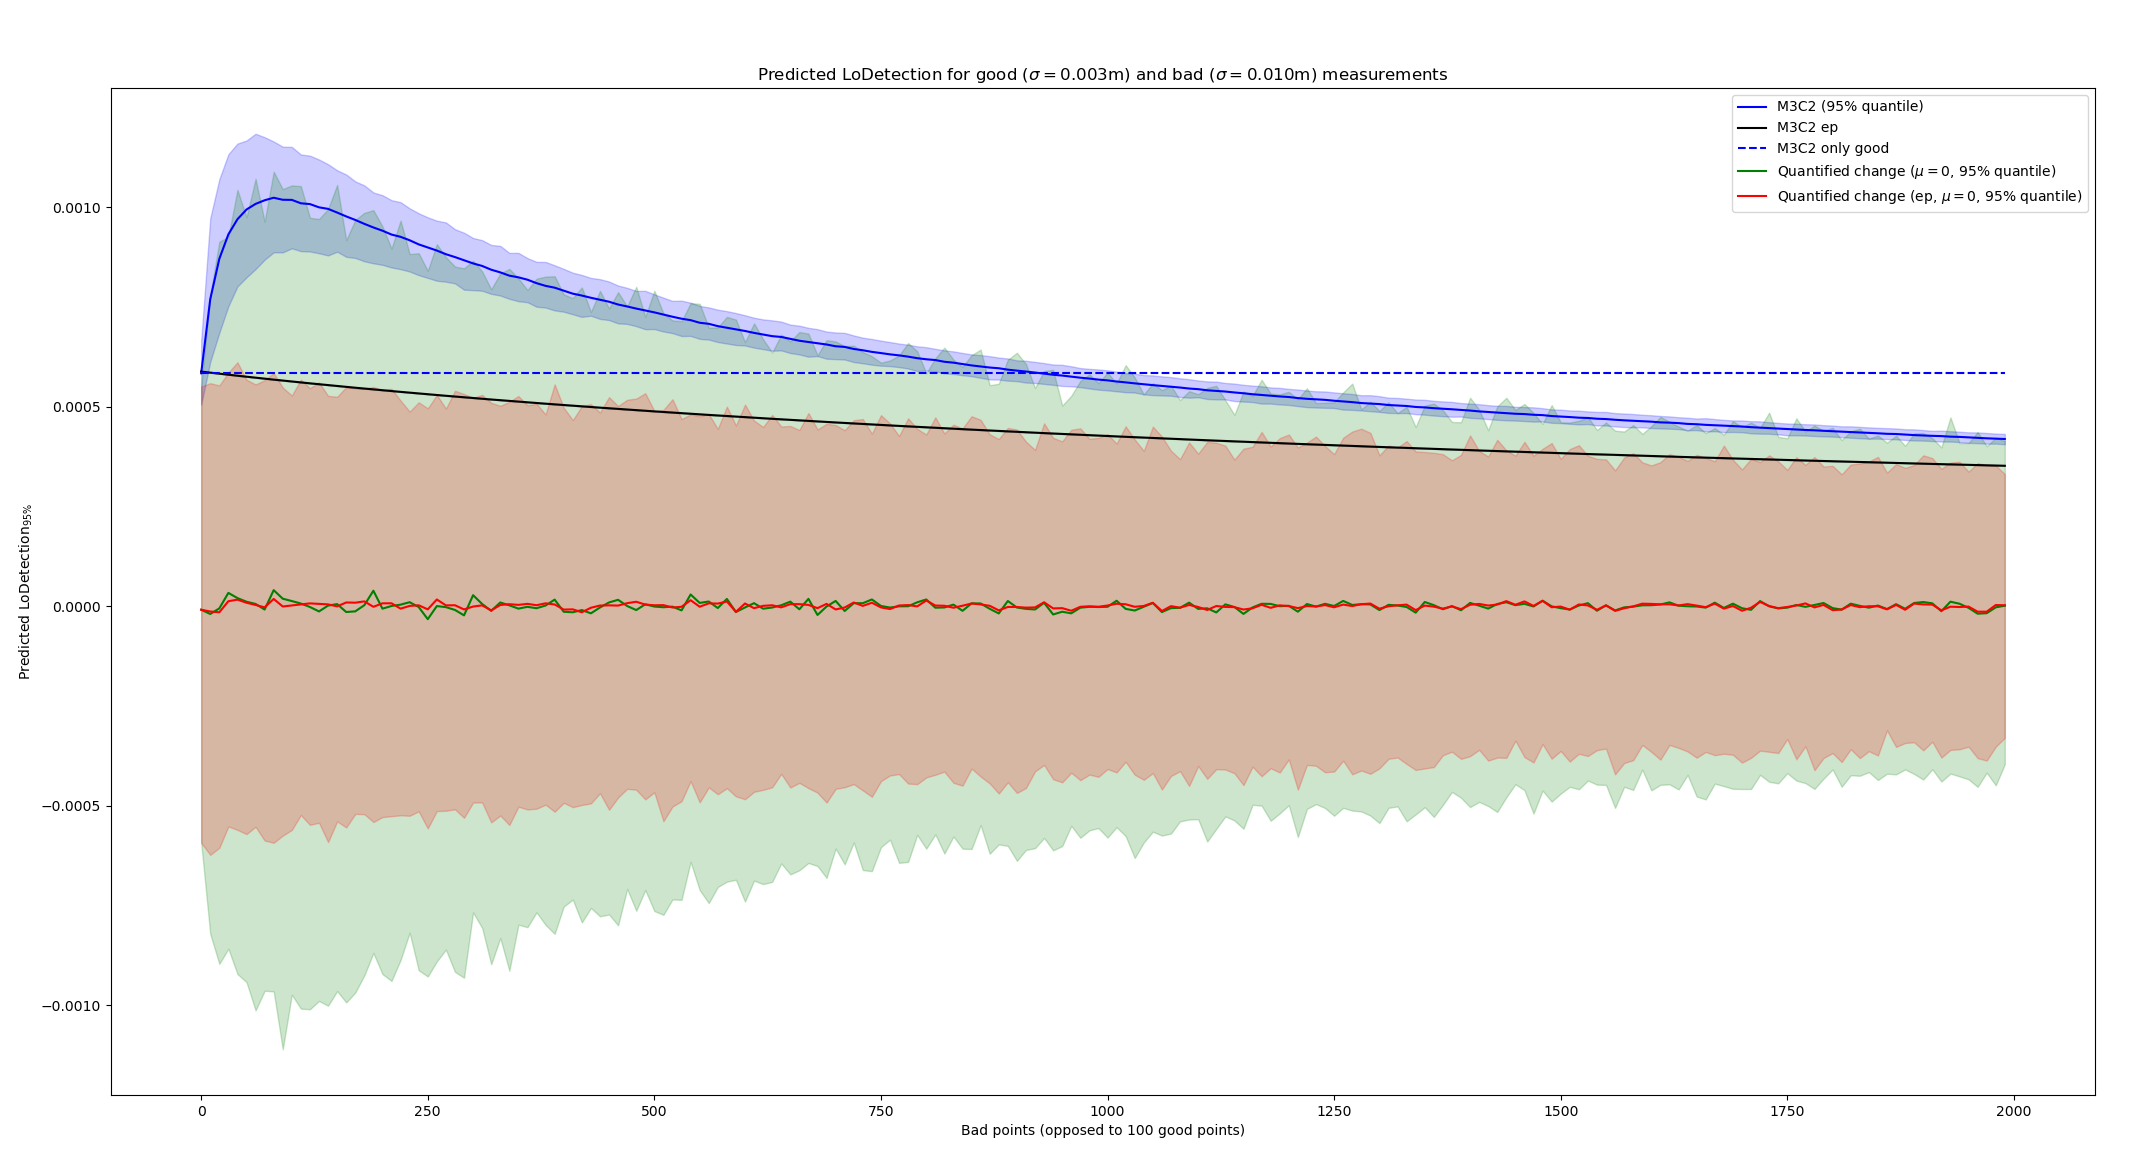
\includegraphics[width=0.9\linewidth]{figs/experiment1.png}
    \caption{Results of simulation with heterogenous point uncertainty}
    \label{fig:plot_a}
\end{figure}

Since the baseline method does not have any information about the a priori uncertainties, the Level of Detection is solely based on the variance calculated from the data itself. This variance increases with the additional points, leading to an increase in the Level of Detection. Only after a significantly higher amount of points, at about 1000 points in total, the Level of Detection decreases to a level lower than with just the 100 points of low uncertainty. This is solely due to the increase in the number of points, which makes the statistical test more sensible.

When filtering points by their variance, e.g. by separating multiple scan positions and only keeping the one with the closest range, the Level of Detection can be kept at a constant level. This approach ignores the additional observations in an attempt not to make the estimation of the Level of Detection worse.

When optimally combining the two sets of observations, by taking a mean weighted by the inverse variances, the Level of Detection from Error Propagation (LoDetection-EP) decreases already with the first added point, even if it has the higher uncertainty. We show this by the black curve, which is always below the blue and the dashed blue lines.

The expectation for the quantified distance in this example is zero, which is also shown by the red and the green lines, representing the distances for the mean and for the weighted mean respectively. By looking at their center 95-percentile (i.e., the range between the 2.5 and the 97.5-percentile), we see a difference between the distribution of the two means, as indicated by the red and green shaded areas. Also, the border of the green shade (non-weighted mean percentile) coincides with the mean Level of Detection (baseline, in blue), and the border of the red shade (weighted mean percentile) with the propagated Level of Detection (LoDetection-EP, in black). This shows the relationships of the confidence (taken to be 95\%) and the quantiles of the estimated distance, i.e. 95\% of the estimations for zero are (by absolute value) lower than the predicted Level of Detection, for both methods.

\subsection{(b) Non-planar objects}
In the second simulated experiment, we consider a laser scanner with a single ranging uncertainty of $\sigma$=0.005 m scanning an edge. The edge is assumed to by symmetric, i.e. the same number of points are scanned on the left and on the right side of the edge. For the change analysis, we again assume a change of zero, and consider the direction facing the scanner as the direction of analysis.

\begin{figure}
    \centering
    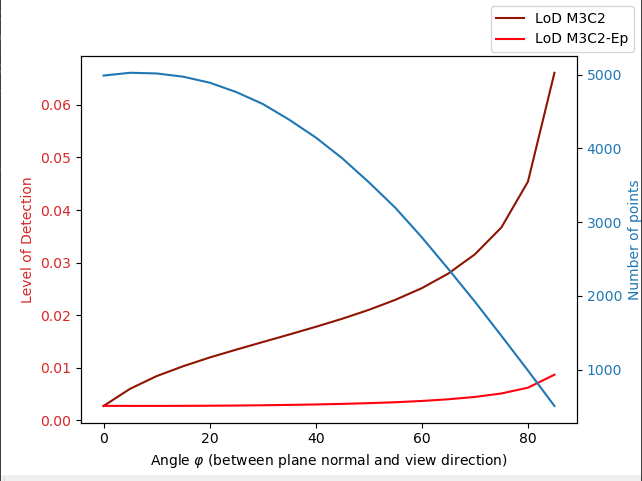
\includegraphics[width=0.9\linewidth]{figs/experiment2.png}
    \caption{Results of simulation of a non-planar object}
    \label{fig:plot_b}
\end{figure}

Figure~\ref{fig:plot_b} shows that with an increasing angle of the edge, the baseline Level of Detection (dark red) increases and tends towards infinity for very sharp edges. Our method, LoDetection-EP (light red), first even shows a decrease in the Level of Detection, as more points are being sampled on the slightly slanted surfaces than on a perfectly flat one, orthogonal to the beam direction. At an incidence angle of about 60 degrees, the LoDetection-EP also starts to increase, but solely based on the decreasing number of points (blue) within the 1 m search radius used for this analysis. The simulation was carried out assuming an infinitesimal footprint, and therefore no influence of the incidence angle on the range measurement. In real-world applications, an increasing incidence would lead to higher ranging uncertainties, as shown e.g. by Soudarissanane (…). However, with this analysis we want to show the effect of non-planar objects for the detection and quantification of change, not the influence on ranging precision per se.
As a validation, we again plot the central 95-percentile of the quantified change (with expectation zero) as the red area, which coincides nicely with the LoDetection-EP, while the baseline overestimates the Level of Detection.  

\subsection{(c) Alignment uncertainty}
\label{sec:results-c}
As presented in Section ??, additional uncertainties stemming from the alignment of the two epochs have to be considered in real-world applications where the scan positions are not fixed (i.e. survey pillars). The baseline method uses a constant coregistration uncertainty for the whole dataset, which we estimate from residual point-to-plane distances in areas that were manually delineated as stable rock. For the coregistration from 2017 to 2018a, the mean residuals were 0.02 m, for the coregistration from 2018a to 2018b, they were XX m.


\begin{figure}
    \centering
    
\includegraphics[width=0.45\linewidth]{placeholder.jpg}
    
\includegraphics[width=0.45\linewidth]{placeholder.jpg}
    \caption{Comparison of influence of measurement (left) and alignment (right) uncertainties on per-point semi-major axes}
    \label{fig:plot_c}
\end{figure}

In contrast to this single measure, we use the uncertainty of the transformation parameters as estimated from the residuals in the ICP alignment. For a full (12-parameter) transformation, this corresponds to a 144-element covariance matrix. 

We first calculate the average covariances for every core point of the AHK rock glacier only based on the alignment uncertainty. For this, we set the measurement uncertainty to zero. Figure ?? shows the results for this analysis, where low uncertainty (blue, ~ ?? mm) appears in the central area of the rock glacier and the adjacent hillslope. The uncertainty gradually increases towards the edges of the dataset and the crevasse at the orographic right edge of the rock glacier (yellow, ~ ?? m).

The smooth gradient of the resulting uncertainty suggests the validity of ignoring between-point correlations for the calculation of the mean coordinates at core point level (Section ??). Additionally, since the Center of Gravity is in the geometric center of the local neighbourhood, linear coregistration effects from points on opposite sides of the neighbourhood cancel each other.

Subsequently, we compare the uncertainty stemming only from the alignment with the one stemming only from the measurement process. Here, shorter ranges and more overlap lead to overall lower uncertainty values on the rock glacier itself (blue, ~ ?? m), and higher uncertainties with longer ranges (yellow, ~ ?? m).


\subsection{(d) Application example}
accuracy (Experiment a), the three-dimensional test based on error propagation (Experiment b) and the influence of the coregistration (Experiment c) to apply our method to the Äußeres Hochebenkar dataset.

Figure ?? shows the predicted Level of Detection using the baseline method and our methods, as well as their difference for the 2017-2018a timespan. Note how the Level of Detection is always lower than the baseline with our methods, meaning that smaller changes can be detected. On average, the improvement in this timespan is ?? m, with values up to ?? m in areas covered by multiple scan positions. Similarly, Figure ?? shows the improvement in the Level of Detection for the 2018a-2018b, three week timespan. 
Since we used the uncertainties also as weights in the calculation of the distance measure (and not only for error propagation and the associated test), the resulting point cloud differences are slightly different. Differences are especially pronounced in narrow channels and at objects where two scan positions with a large difference in range overlap. Figure ?? shows the difference in the change value for the 2018a-2018b timespan.
 
\begin{figure}
    \centering
    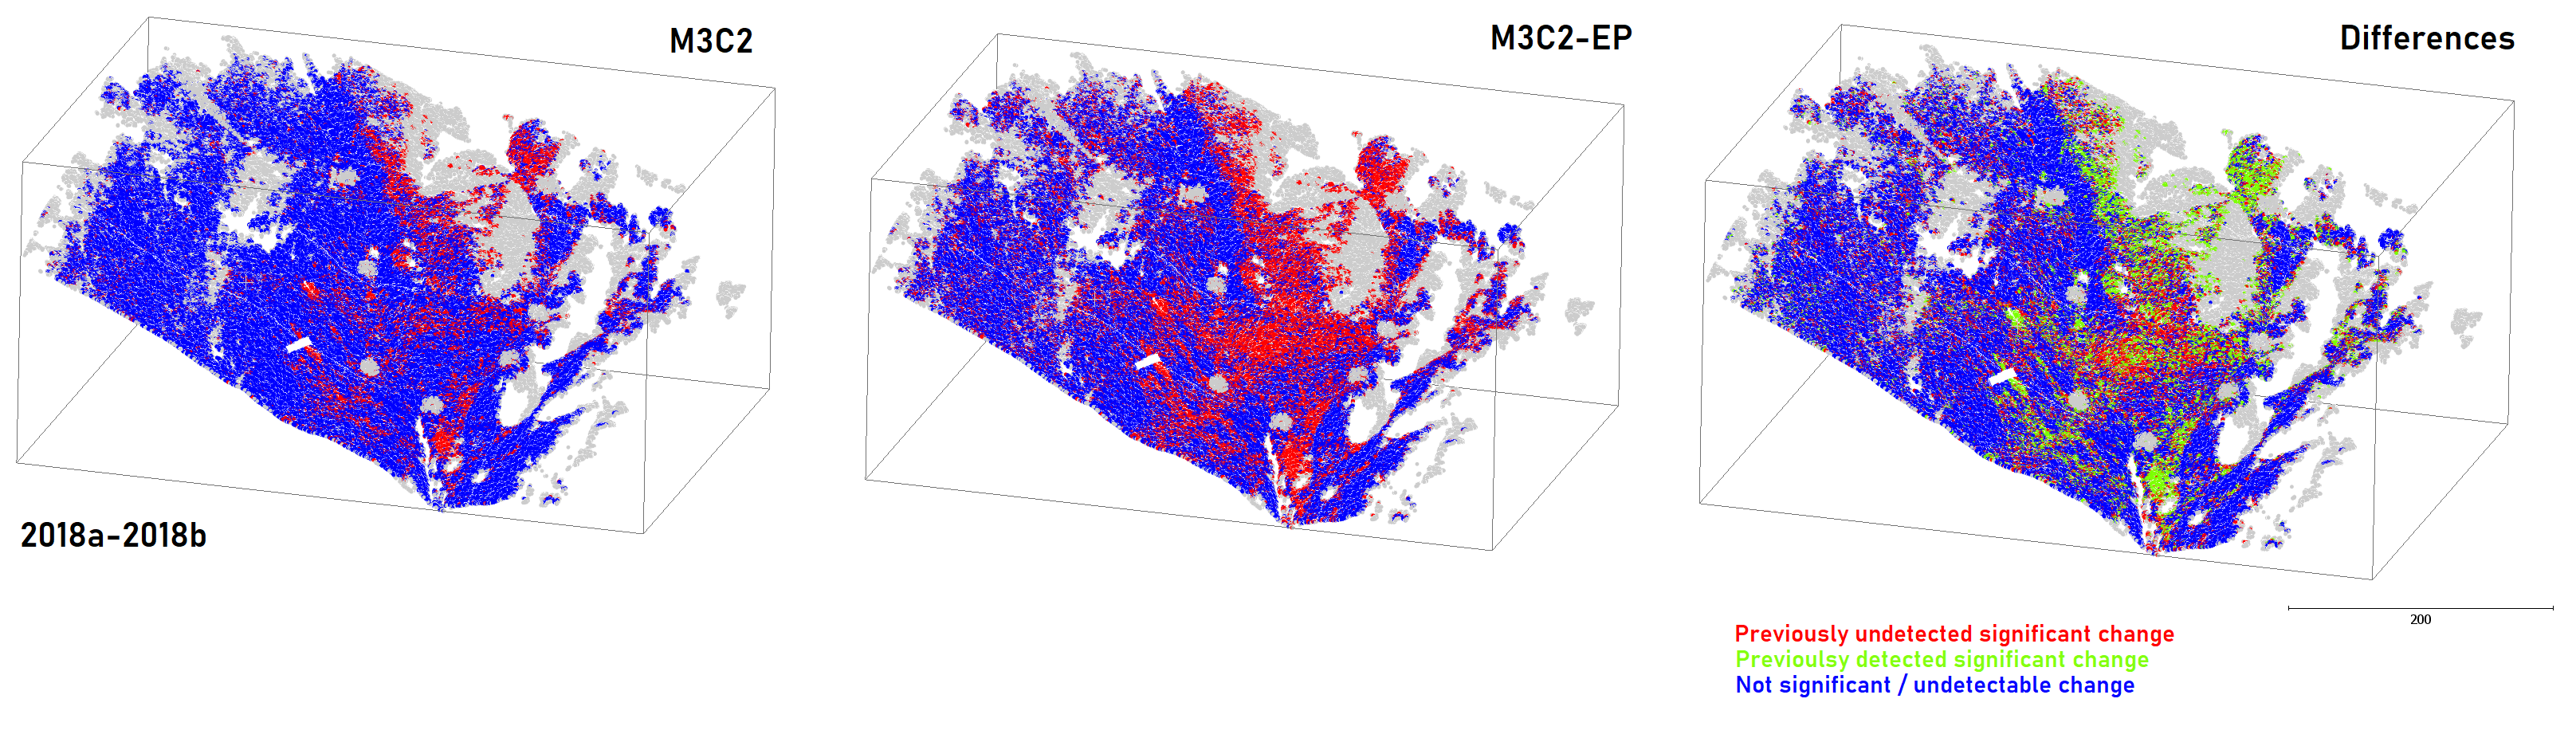
\includegraphics[width=0.9\linewidth]{figs/result_sig_change_2018ab.png}
    
\includegraphics[width=0.3\linewidth]{placeholder.jpg}
\includegraphics[width=0.3\linewidth]{placeholder.jpg}
\includegraphics[width=0.3\linewidth]{placeholder.jpg}
    \caption{}
    \label{fig:plot_d}
\end{figure}
 
To separate noise in these difference values from real change, the Level of Detection is used as a threshold. For the baseline, we compare the predicted Level of Detection with the M3C2 distance, and for our method, we use the weighted M3C2-EP distance thresholded by the Level of Detection from error propagation. We show the result as a binary change map for both methods and both timespans in Figure~\ref{fig:plot_d} (a-d) and the differences in change detection between the two methods in Figure~\ref{fig:plot_d} (e, f).
 
 The red points in Figure~\ref{fig:plot_d} (e, f), representing change that was deemed indistinguishable from noise with the baseline method, but detectable change with our method, amount to 18\% of the total area of interest, or an increase in core points with detected change by 53\% (from 15\% to 23\%) of the total core points for the 2018a-2018b timespan; and to ??\% (an increase by ??\%; from ??\% to ??\% of the total core points) for the 2017-2018a timespan. There are no core points that were previously deemed significant and changed to not significant with our method, supporting the claims of the overestimation of the Level of Detection by M3C2.
 
When multiplying the change values at the locations that were previously not detected but give significant change with our method with some area (e.g. the base of the cylinder, if this matches the core point sampling), we can estimate the volume of change that was missed by the baseline method. In the 2018a-2018b timespan and using a base area of $A=r^2\pi=0.126m^2$ this amounts to 217.72 $m^3$, of a total change volume of 734.83 $m^3$ (30\%). For the 2017-2018a timespan, the additional volume is ?? $m^3$ of ?? $m^3$, which is ??\%. Please note that these values are not an accurate representation of moved rock mass, as they also include vegetation and other effects, and the search cylinders may overlap at concave locations, leading to an overestimation. 

The volume change difference is (at 30\% for the 2018a-2018b timespan) a bit smaller than the difference in the number of core points (at 35\%), which is due to the large change values already being detected by the baseline method, and the improvement mainly representing points with smaller changes.

Since there is no ground truth data for real change on the rock glacier, we estimate the accuracy of our change detection method by investigating the original point clouds at exemplary locations, especially where our method differs from the baseline. 

Examples:

\begin{figure}
    \centering
    
\includegraphics[width=0.45\linewidth]{placeholder.jpg}
    
\includegraphics[width=0.45\linewidth]{placeholder.jpg}
    \caption{Directionality in the analysis, non-planar areas}
    \label{fig:example_1}
\end{figure}
\begin{figure}
    \centering
    
\includegraphics[width=0.45\linewidth]{placeholder.jpg}
    
\includegraphics[width=0.45\linewidth]{placeholder.jpg}
    \caption{Vegetation is significant}
    \label{fig:example_2}
\end{figure}
\begin{figure}
    \centering
    
\includegraphics[width=0.45\linewidth]{placeholder.jpg}
    
\includegraphics[width=0.45\linewidth]{placeholder.jpg}
    \caption{High LoD but lower change}
    \label{fig:example_3}
\end{figure}

 \begin{itemize}
    \item Directionality
    \item Vegetation (also in 3 weeks!) – could be removed beforehand
    \item Where change is “just below” LoD? (high LoD)
 \end{itemize}

\section{Discussion}
In our analyses, we used a constant search radius for both the normal vector calculation and the cylinder projection. The significance of the change results for the geomorphic analysis of the rock glacier may suffer from this simplification, but the focus on this study was to compare the M3C2 baseline method with our extension, M3C2-EP. The significance of the results presented in Section ?? are not influenced by the search radius, as we used the same radius for both methods. 

Closely related yet separate is the question of the direction of change analysis. Using the local surface normal vector is applicable for many processes but can lead to hard to interpret results e.g. at a rock fall where the local surface changes significantly. Williams et al. (in review) analyze change in 60 different directions and at different scales to find the direction of mean displacement (DMD). M3C2-EP allows yet a different approach. By applying an eigenvalue decomposition on the propagated covariance matrix, the direction in which change can be best detected can be calculated. While is direction is not motivated by geomorphic processes, it allows for optimization of the measurement setup to align this direction e.g. with the DMD. Such an optimization can be achieved by using laser scanning simulation software to automatically try different scan positions and -settings, such as the HELIOS software (Bechtold \& Höfle, 2013).

The amount of core points that can be attributed significant change instead of noise increased for both timespans with our method. As expected, this was especially prominent for the shorter timespan of 3 weeks (2018a-2018b), where changes are in general smaller. Therefore, a lower Level of Detection is required to detect the changes that are present. 
Changes that we detect as significant but were overlooked by the baseline method mostly concern vegetation, where the planarity assumption of M3C2 is violated. This may be overcome by filtering vegetation from the point cloud in a preprocessing step.

Nevertheless, in the alpine terrain of the Äußeres Hochebenkar, the surface can be quite rough at the projection radius scale, which leads to an overestimation of the M3C2 Level of Detection as shown in Experiment (b). Examples of boulders on and around the rock glacier show the validity of our method for these cases. Such high roughness is especially prominent at locations of active mass movements, as new surfaces form that have not exposed to weathering events for some time prior to the analysis.


\section{Conclusion}
In this paper, we presented an addition to the state-of-the-art 3D point cloud distance metric M3C2 by applying error propagation, called M3C2-EP. M3C2-EP extends M3C2 by allowing the estimation of uncertainty values for every point in a 3D point cloud, which can be used to distinguish significant change from noise. We use knowledge about the sensor that acquired the data (i.e. measurement uncertainty) and the alignment of the two datasets (by a full covariance metric stemming from the ICP algorithm) to estimate the M3C2-EP Level of Detection.

Two simulated experiments show the validity of the method in two cases where the baseline M3C2 grossly overestimates the Level of Detection, namely the overlap of measurements with different uncertainties and the analysis of non-planar objects. Monte-Carlo simulations further proof the correctness of our adapted significance test based on Hotelling’s T-squared distribution for equal multivariate means. We also show that the calculation of the distance between the point clouds must be based on the same per-point weights derived from the propagated uncertainties.

While our approach requires the input of additional metadata, such as the sensor accuracy, alignment information, and the scan positions (or trajectory for a dynamic scan), we achieve on average ??\% lower values for the Level of Detection for an analysis of a real dataset in the Austrian alps over a  timespan of 3 weeks. This corresponds to 53\% more areas where change could be significantly quantifies, and 217 m³ additional change volume (30\% of the total change volume) when compared to the baseline. 

The significance of M3C2-EP especially shows in rough areas, such as areas that are influenced by active geomorphic events. These lead to the formation of new surfaces that have not been exposed to weathering effects for a long time and therefore violate M3C2’s planarity assumption. Additionally, our approach allows the combination of datasets with different accuracies (e.g. multiple scan positions with different ranges) without degradation of the resulting Level of Detection. Especially when combining different sensors, platforms (terrestrial, airborne) and methods (laser scanning, photogrammetric image matching), this consideration is important to use all datasets to their full capacity.

In light of recent trends towards 4D analyses, such as (Anders et al., 2020), consideration of measurement and alignment uncertainties are becoming more important, as some epochs may be recorded by instruments with higher uncertainties (such as low-cost sensors, Eltner et al., ??) and complemented in regular intervals by high-precision sensors. When estimating e.g. a trend, the knowledge of uncertainty can be leveraged to get a more reliable result.


%% The Appendices part is started with the command \appendix;
%% appendix sections are then done as normal sections
%% \appendix

%% \section{}
%% \label{}

%% References
%%
%% Following citation commands can be used in the body text:
%% Usage of \cite is as follows:
%%   \cite{key}          ==>>  [#]
%%   \cite[chap. 2]{key} ==>>  [#, chap. 2]
%%   \citet{key}         ==>>  Author [#]

%% References with bibTeX database:

%%\bibliographystyle{model1-num-names}

%% New version of the num-names style
\bibliographystyle{elsarticle-num-names}
\bibliography{sample.bib}

%% Authors are advised to submit their bibtex database files. They are
%% requested to list a bibtex style file in the manuscript if they do
%% not want to use model1-num-names.bst.

%% References without bibTeX database:

% \begin{thebibliography}{00}

%% \bibitem must have the following form:
%%   \bibitem{key}...
%%

% \bibitem{}

% \end{thebibliography}


\end{document}

%%
%% End of file `elsarticle-template-1-num.tex'.